% =====================================================================================================
%  IEEE Access manuscript, official IEEE Access LaTeX template (ieeeaccess.cls, 2023 release, Formata fonts).
%  Build with pdfLaTeX:  pdflatex main && bibtex main && pdflatex main && pdflatex main
%  Supplementary material: supplement.tex (separate PDF).
%  Items marked \TODO{} need data or decisions from the authors (see ../REVIEW_RESPONSE.md).
% =====================================================================================================
\documentclass{ieeeaccess}
\usepackage{cite}
\usepackage{amsmath,amssymb,amsfonts}
\usepackage{algorithm}
\usepackage{algpseudocode}
\usepackage{graphicx}
\usepackage{textcomp}
\usepackage{booktabs}
\usepackage{multirow}
\usepackage{array}
\usepackage{xcolor}
\usepackage{url}
\def\BibTeX{{\rm B\kern-.05em{\sc i\kern-.025em b}\kern-.08em
    T\kern-.1667em\lower.7ex\hbox{E}\kern-.125emX}}

\newcommand{\TODO}[1]{\textcolor{red}{[TODO: #1]}}
\newcommand{\gold}{$\mathcal{G}_{58}$}
\algrenewcommand\algorithmicrequire{\textbf{Input:}}
\algrenewcommand\algorithmicensure{\textbf{Output:}}

\begin{document}
\history{Date of publication xxxx 00, 0000, date of current version xxxx 00, 0000.}
\doi{10.1109/ACCESS.2026.DOI}

\title{Report-Supervised Distillation for Multi-Label Knee MRI Classification: An Evaluation Under Limited Expert Annotation}

\author{\uppercase{Md. Hamid Hosen}\authorrefmark{1},
\uppercase{Md. Foysal Emon Shanto}\authorrefmark{2},
\uppercase{Md Esfer Abdus Sami}\authorrefmark{3}, and
\uppercase{\TODO{Author 4 full name (Kaggle: kishormorol)}}\authorrefmark{4}}

\address[1]{Department of Computer Science and Engineering, East Delta University, Chattogram, Bangladesh (e-mail: mdhamidhosen4@gmail.com)}
\address[2]{Department of Computer Science and Engineering, Jashore University of Science and Technology, Jashore, Bangladesh (e-mail: foyshalsk348@gmail.com)}
\address[3]{Department of Computer Science and Engineering, North South University, Dhaka, Bangladesh (e-mail: esfer.sami.me@gmail.com)}
\address[4]{\TODO{Department, University, City, Country} (e-mail: \TODO{e-mail})}

\tfootnote{\TODO{Funding statement, or ``This work did not receive external funding.''}}

\markboth
{Hosen \headeretal: Report-Supervised Distillation for Multi-Label Knee MRI Classification}
{Hosen \headeretal: Report-Supervised Distillation for Multi-Label Knee MRI Classification}

\corresp{Corresponding author: Md. Hamid Hosen (e-mail: mdhamidhosen4@gmail.com).}

\begin{abstract}
Expert image-level labels are scarce for multi-label knee MRI, whereas radiology reports are abundant. We ask how
report-consensus targets, self-distillation and distillation from an external image-input model affect a study-level
classifier when only 58 of 4,407 training studies carry expert labels for 12 findings (RSNA Knee Abnormality dataset).
A publicly available 2.5D ConvNeXt reader was trained on (i) the mean of four language-model report labellers,
(ii) a mixture of these labels with its own out-of-fold predictions, and (iii) mixtures with a public CoAtNet teacher
whose training used report labels and, for three findings, expert MRI grades from an external cohort. On a 385-study
development partition of the hidden test set, which also informed model development, the three targets gave macro ROC
AUCs of 0.933, 0.939 and 0.948--0.949; the teacher displayed 0.949. Changes of backbone, pre-training and seed showed no
clear benefit in the configurations evaluated. Rank fusion of the students with public ensembles ranked above the
unchanged parent in eight of eight development comparisons. On the held-out 70\% final-test partition, matched parents
with and without students scored \TODO{x.xxx--x.xxx vs. x.xxx--x.xxx}, and the readers A, B and C3 scored \TODO{}. Bootstrap intervals on the 58 expert-labelled studies were
about 0.05 wide, and a simulation illustrates that a partition of this size can mis-order models whose AUCs differ by
about 0.001. Development comparisons are therefore exploratory. Code and experiment logs are released.
\end{abstract}

\begin{keywords}
Knee MRI, knowledge distillation, multi-label classification, pseudo-labelling, radiology reports, weak supervision,
model evaluation.
\end{keywords}

\titlepgskip=-21pt

\maketitle

% =====================================================================================================
\section{Introduction}
\label{sec:intro}

\PARstart{K}{nee} MRI is the reference non-invasive examination for internal derangement of the knee, and a single study
is expected to address ligaments, menisci, cartilage in three compartments, joint fluid, the synovium, popliteal cysts and
bone marrow. Deep learning has matched radiologists on single tasks such as anterior cruciate ligament (ACL) and meniscal
tears and cartilage lesions~\cite{bien2018mrnet,liu2018cartilage,pedoia2019meniscus,namiri2020acl,fritz2020meniscus},
and multi-finding models have been trained on expert-annotated cohorts~\cite{astuto2021knee,qiu2024coplane}. These
systems depend on image-level labels from expert readers, which are costly to obtain at scale.

Radiology reports are abundant but are an imperfect proxy: radiologists omit findings they consider irrelevant, hedge,
and grade severity in free text. The RSNA Knee Abnormality dataset~\cite{rsna2026knee} makes the gap explicit. Of its
4,407 training studies, all have a report, and 58 additionally have expert labels for 12 findings, which the organisers
stated were produced by an image-based process independent of the reports. A model trained on report labels is
therefore optimised for a target that differs from the one used to evaluate it.

This paper addresses one question: \emph{under limited expert annotation, how do report consensus, self-distillation and
external image-model distillation affect knee MRI classification?} Our hypothesis was that the training target, rather
than the backbone, limits a report-supervised reader. The contributions are:
\begin{enumerate}
\item A controlled comparison of training targets for a fixed 2.5D reader---report consensus, out-of-fold
self-distillation, and an external image-input teacher at two mixing weights---with every change logged prospectively as
a single variable against a scored parent (Sections~\ref{sec:method-distill} and~\ref{sec:res-distill}).
\item An evaluation of whether such students add information to strong existing ensembles, on the development partition
and on the held-out final-test partition (Sections~\ref{sec:res-final} and~\ref{sec:res-ens}).
\item An analysis of what the available evaluation data can resolve, with negative results on models whose
out-of-fold performance did not translate into ensemble benefit (Sections~\ref{sec:res-own} and~\ref{sec:res-yard}).
\end{enumerate}

\paragraph*{What was reused} The reader architecture, its preprocessing and its training code were released
publicly by another author~\cite{goodpjw2026reader}; the report label tables~\cite{labels2026public}, the teacher
models~\cite{nartaa2026mirror,heliosli2026blend} and the ensembles used for fusion~\cite{heliosli2026blend,goodpjw2026stack}
are likewise public. Our work is the experimental design, the target and teacher comparisons, the fusion experiments,
the analyses, and implementation changes needed to run them (Fig.~\ref{fig:overview}).

\begin{figure*}[!t]
\centering
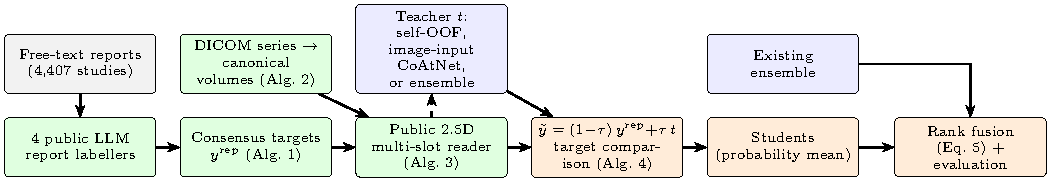
\includegraphics[width=\textwidth]{figures/overview.pdf}
\caption{Overview. Green: reused public components (report labels, preprocessing and reader architecture); blue: external
teachers and ensembles; orange: components of this work (target construction and comparison, fusion, evaluation). The
dashed arrow denotes self-distillation, in which the teacher is the reader's own out-of-fold prediction.}
\label{fig:overview}
\end{figure*}

% =====================================================================================================
\section{Related Work}
\label{sec:related}

\subsection{Deep learning for knee MRI}
MRNet~\cite{bien2018mrnet} applied per-plane 2D CNNs with slice pooling to abnormality, ACL-tear and meniscal-tear
detection; ELNet~\cite{tsai2020elnet} proposed a lighter slice-wise network. Task-specific models address cartilage
lesions~\cite{liu2018cartilage}, meniscal and patellofemoral degeneration~\cite{pedoia2019meniscus}, ACL
severity~\cite{namiri2020acl} and meniscal tears with a surgical reference~\cite{fritz2020meniscus,roblot2019meniscus}.
Astuto et al.~\cite{astuto2021knee} graded several tissues in one pipeline, and Qiu et al.~\cite{qiu2024coplane}
diagnosed twelve knee abnormalities with co-plane attention across sequences (overall AUC 0.812 on 1,748 subjects).
External cohorts---the Osteoarthritis Initiative (OAI)~\cite{peterfy2008oai}, fastMRI~\cite{zbontar2018fastmri},
SKM-TEA~\cite{desai2021skmtea}---and radiology pre-training~\cite{mei2022radimagenet} are widely used. All of these
works rely on image-level labels for the target task, which our setting largely lacks.

\subsection{Learning from radiology reports}
Rule-based~\cite{wang2017chestxray8,irvin2019chexpert} and transformer~\cite{smit2020chexbert} report labellers
produced the first large chest radiograph datasets, and LLMs can structure free-text reports~\cite{adams2023gpt4}. For
spinal MRI, image classifiers trained on LLM-extracted report labels performed comparably to classifiers trained on
clinician annotations~\cite{park2024spinal}. Report labels inherit omissions and hedging, which CheXpert handled with an
uncertainty class~\cite{irvin2019chexpert}.

\subsection{Pseudo-labelling and distillation}
Knowledge distillation trains a student on a teacher's soft outputs~\cite{hinton2015distilling}; born-again
networks~\cite{furlanello2018born} and Noisy Student~\cite{xie2020noisy} showed that students of similar capacity can
match or exceed their teachers. Pseudo-labelling~\cite{lee2013pseudo} and bootstrapped targets that mix noisy labels with
predictions~\cite{reed2015bootstrapping} are close relatives; our targets are of the latter form.

\subsection{Closest work on this dataset}
Kooklan~\cite{kooklan2026gap} analysed the same dataset and compared report-derived targets with the out-of-fold
predictions of a public image model against the 58 expert-labelled studies. The report labels and the image model reached
similar agreement with the experts (macro AUC 0.892 and 0.896) but failed on different findings, and their equal mixture
agreed better (0.927). However, a 2.5D ResNet-50 trained on the mixture did \emph{not} outperform the same model trained on
report labels on the final-test partition (0.872 vs 0.877). Our study differs in the reader (a 2.5D multi-slot ConvNeXt
transformer), in the teachers (an in-sample CoAtNet teacher with external expert grades, and a self-teacher), in the
evaluation of fusion with ensembles, and in its development-partition result, which points the other way. Reconciling
the two findings requires final-test scores of our students (Section~\ref{sec:res-final}).

\subsection{Evaluation with small or hidden test sets}
Repeated evaluation on a fixed partition invites adaptive over-fitting~\cite{blum2015ladder}, although its extent is often
smaller than feared~\cite{roelofs2019meta}. Rankings in biomedical challenges are sensitive to test sampling and metric
choice~\cite{maierhein2018rankings}, and small test sets are a recurring methodological
failure~\cite{varoquaux2022failures}. We report the reporting items of the CLAIM checklist~\cite{claim2024} in the
Supplementary Material.

% =====================================================================================================
\section{Data}
\label{sec:data}

\subsection{Cohort, reference standard and label definitions}
The RSNA Knee Abnormality dataset~\cite{rsna2026knee} is an international, multilingual collection of knee MRI
examinations, each paired with its original radiology report~\cite{chen2026overview}. It contains 4,407 de-identified
training studies (24,371 DICOM series) and a hidden test set of about 1,284 studies. Twelve binary findings are scored
per study under the organisers' names: ACL, MCL, medial meniscus, lateral meniscus, medial OA, lateral OA,
patellofemoral (PF) OA, effusion, synovitis, Baker's cyst, contusion and fracture. Each series carries its plane and a
fat-suppression (FS) flag; Fig.~\ref{fig:illus} illustrates the planes and sequence types with openly licensed images,
because the dataset's terms forbid publishing its images.

\begin{figure*}[!t]
\centering
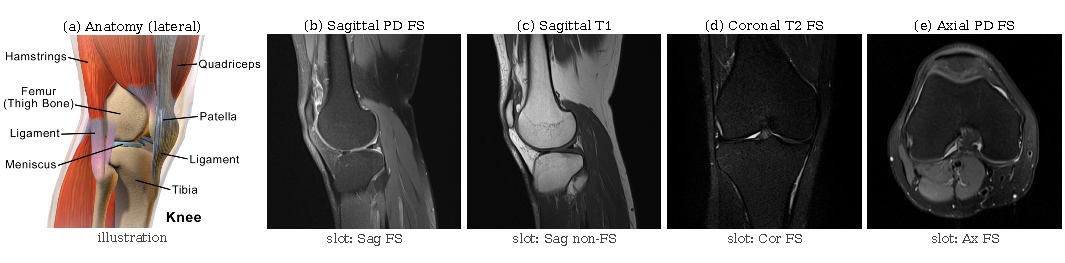
\includegraphics[width=\textwidth]{figures/illustrative_mri.pdf}
\caption{Illustration of knee anatomy and of the MRI planes and sequences that map to the reader's slots
(Section~\ref{sec:method-reader}). \emph{These images are not from the RSNA dataset}, whose terms forbid publishing it.
(a)~Blausen.com staff, ``Medical gallery of Blausen Medical 2014,'' \emph{WikiJournal of Medicine}, 2014,
doi:10.15347/wjm/2014.010, CC~BY~3.0. (b)--(e)~Knee MRI, Siemens MAGNETOM Aera 1.5\,T, by Ptrump16 via Wikimedia Commons,
CC~BY-SA~4.0; (d) and (e) are middle frames of the published coronal and axial series. Cropped and arranged; this figure
is licensed CC~BY-SA~4.0.}
\label{fig:illus}
\end{figure*}

\paragraph*{Reference standard} According to the organisers~\cite{chen2026overview}, every study in the reference set was
labelled independently by two subspecialty-trained musculoskeletal radiologists against a written annotation rubric,
with disagreements adjudicated by a third radiologist; labels apply to the whole examination of a single knee. The
organisers stated separately that the same process was used for the test set~\cite{chen2026clarification}. Borderline findings were graded negative to favour specificity.
Table~\ref{tab:defs} summarises the rubric. Several definitions are narrower than the clinical terms: the ``ACL'' and
``MCL'' targets are high-grade tears, ``OA'' requires high-grade cartilage loss over about 1~cm or more, and effusion and
Baker's cyst must be at least moderate. Reports describe milder grades, which is one source of the report--reference gap
(Section~\ref{sec:data-eda}).

\begin{table}[!t]
\centering
\caption{Positive definitions of the reference labels, summarised from the organisers' annotation rubric~\cite{chen2026overview}.
Borderline findings are negative.}
\label{tab:defs}
\footnotesize
\setlength{\tabcolsep}{3pt}
\begin{tabular}{p{1.9cm}p{6.0cm}}
\toprule
Finding & Positive if\\
\midrule
ACL & high-grade partial ($>$50\% of fibres) or complete tear; signal change or thickening alone is negative\\
MCL & high-grade partial or complete acute tear with fibre disruption and edema; low-grade sprain or chronic change is negative\\
Medial / lateral meniscus & signal definitely reaching the meniscal surface on $\geq$2 images, or a truncated, diminutive or displaced fragment; intrasubstance degeneration is negative\\
Medial / lateral / PF OA & moderate or large area ($\gtrsim$1~cm) of cartilage loss $>$50\% of thickness in that compartment\\
Effusion & moderate or large joint fluid distending the joint\\
Synovitis & inflammation and thickening of the synovial lining\\
Baker's cyst & moderate or large fluid collection in the popliteal location\\
Contusion & bone-marrow edema-like signal from impact without a fracture line\\
Fracture & acute cortical break or fracture line\\
\bottomrule
\end{tabular}
\end{table}

\paragraph*{What is not reported} The materials available to us do \emph{not} report the contributing institutions,
acquisition period, demographics, scanner vendors and field strengths, inclusion and exclusion criteria, patient
identifiers, repeated or bilateral examinations, or how the 58 reference studies were chosen. We mark these items as
unavailable in the CLAIM checklist rather than infer them. Grouping studies with identical reports
(Section~\ref{sec:method-labels}) removes duplicated reports but does not establish patient-level separation.

\subsection{The 58 expert-labelled studies}
\label{sec:data-gold}
Expert labels are available for 58 training studies (\gold). The set is enriched: every study has at least one positive
finding, with 4.14 on average (Table~\ref{tab:gold}). \gold{} was never used for gradient updates of any model trained in
this work. It was, however, used during development: (i) as a diagnostic reported for every model; (ii) as part of some
adoption rules, for example ``adopt a student only if its \gold{} AUC is at least 0.9127'' or ``reject a change if \gold{}
falls by more than 0.01''; and (iii) by the authors of the external teacher, who used it for model
selection~\cite{nartaa2026mirror}. Its scores and intervals are therefore descriptive development results, not
independent estimates.

\begin{table}[!t]
\centering
\caption{Positive studies per finding in the 58 expert-labelled studies (\gold).}
\label{tab:gold}
\setlength{\tabcolsep}{3pt}
\begin{tabular}{lc@{\hskip 8pt}lc@{\hskip 8pt}lc}
\toprule
Finding & $n_+$ & Finding & $n_+$ & Finding & $n_+$\\
\midrule
ACL & 24 & Medial OA & 15 & Synovitis & 27\\
MCL & 9 & Lateral OA & 11 & Baker's cyst & 12\\
Med. meniscus & 26 & PF OA & 21 & Contusion & 19\\
Lat. meniscus & 23 & Effusion & 35 & Fracture & 18\\
\bottomrule
\end{tabular}
\end{table}

\subsection{Report-derived labels}
Several groups released LLM-extracted labels for all training studies~\cite{labels2026public}; for example, the number
of fracture-positive studies ranges from 159 to 336 across five tables. Table~\ref{tab:labels} compares two label sets on
the 4,349 studies outside \gold: \emph{set~D}, the soft labels \texttt{labels\_llm\_soft} of
dreaddevelopment~\cite{dread2026raptor}, used by our EfficientNetV2-S models (Section~\ref{sec:res-own}); and \emph{set~T}, a
team consensus of four public tables (Section~\ref{sec:data-eda}). Neither is the reader's target v0
(Section~\ref{sec:method-labels}). The table measures agreement between label sources, not accuracy against expert labels. The
two sets order studies similarly for 11 findings (AUC 0.89--0.99) but not for synovitis (0.62), because one imputes
synovitis from effusion when the report is silent. For effusion the disagreement is a threshold: ``small effusion'' is
about 0.2 in one set and 0.85 in the other, which flips 34\% of studies at 0.5 while preserving their order.

\begin{table}[!t]
\centering
\caption{Agreement between two report-derived label sets on 4,349 training studies (inter-source agreement, not accuracy):
AUC of set~D against set~T binarised at 0.5, Cohen's $\kappa$ at 0.5, and positive rates ($\geq0.5$) of each set.}
\label{tab:labels}
\setlength{\tabcolsep}{4pt}
\begin{tabular}{lcccc}
\toprule
Finding & AUC & $\kappa$ & D pos. & T pos.\\
\midrule
ACL & 0.950 & 0.70 & 0.13 & 0.21\\
MCL & 0.983 & 0.44 & 0.05 & 0.15\\
Medial meniscus & 0.966 & 0.84 & 0.38 & 0.42\\
Lateral meniscus & 0.967 & 0.80 & 0.14 & 0.16\\
Medial OA & 0.979 & 0.69 & 0.25 & 0.37\\
Lateral OA & 0.969 & 0.61 & 0.15 & 0.27\\
PF OA & 0.987 & 0.73 & 0.34 & 0.46\\
Effusion & 0.919 & 0.38 & 0.26 & 0.60\\
Synovitis & \textbf{0.619} & 0.31 & 0.25 & 0.13\\
Baker's cyst & 0.986 & 0.59 & 0.12 & 0.25\\
Contusion & 0.891 & 0.55 & 0.15 & 0.17\\
Fracture & 0.979 & 0.68 & 0.04 & 0.07\\
\midrule
Macro & 0.933 & 0.61 & & \\
\bottomrule
\end{tabular}
\end{table}

\subsection{Exploratory analysis of the labels}
\label{sec:data-eda}
We analysed the labels that were available locally (no images). The source tables of the reader's target v0 are not
stored in our repository, so Figs.~\ref{fig:shares}--\ref{fig:perstudy} use a \emph{different} construction: set~T, a
team consensus of four public tables (mri-balanced-labels-public, jev-knee-labels \texttt{HYBRID\_labels\_scores},
hybrid-report-labels \texttt{report\_labels\_v4hybrid} and stevenleehans \texttt{llm\_labels\_v4\_blend}), which were
accepted because their \gold{} macro AUC was within 0.03 of the best table; one post-processing rule (a cap on medial OA
when the report is silent) was also kept because it raised \gold{} AUC~\cite{hack2publish2026repo}. Set~T shares one
source with v0 and was used for training only by the E03b model. These figures therefore describe report-derived labels
in this cohort, not the reader's training targets, and set~T's agreement with \gold{} is not reported because \gold{}
shaped it. Fig.~\ref{fig:labellers} uses a benchmark of public tables against \gold{} computed by the same pipeline.

\paragraph*{Label composition} Fig.~\ref{fig:shares} shows, for each finding, the share of studies whose set-T label
is negative ($<0.25$), uncertain (0.25--0.7) or positive ($\geq0.7$). Positive shares range from 5\% (fracture) to 58\%
(effusion). Synovitis is the most ambiguous finding: 49\% of studies fall in the uncertain band, compared with 4--21\% for
the other findings, in line with its low inter-source agreement (Table~\ref{tab:labels}).

\begin{figure}[!t]
\centering
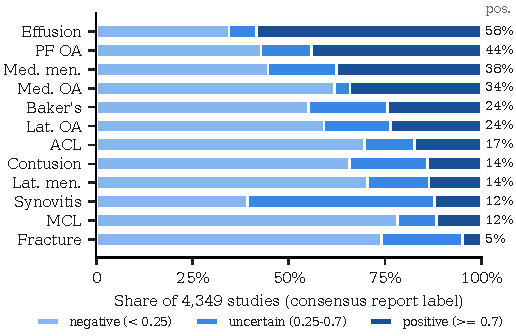
\includegraphics[width=\columnwidth]{figures/label_shares.pdf}
\caption{Composition of the team-consensus labels (set~T; not the reader's targets v0) of the 4,349 report-labelled studies, by finding. Right: positive share.}
\label{fig:shares}
\end{figure}

\paragraph*{Co-occurrence} Findings co-occur in clinically expected patterns (Fig.~\ref{fig:cooc}): effusion and synovitis
($r=0.67$), the three OA compartments (0.57--0.61), contusion and fracture (0.50), and medial meniscus with medial OA (0.47);
ACL is most associated with contusion (0.43) and MCL (0.33). These dependencies are one reason why a shared study
representation with per-finding attention, rather than 12 independent models, is a natural design.

\begin{figure}[!t]
\centering
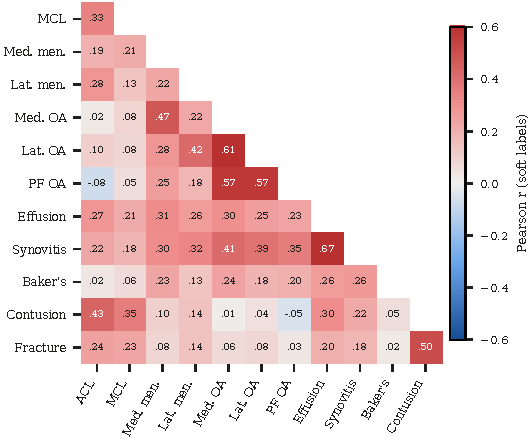
\includegraphics[width=0.92\columnwidth]{figures/label_cooccurrence.pdf}
\caption{Pearson correlation between the team-consensus soft labels (set~T) of the 12 findings (4,349 studies).}
\label{fig:cooc}
\end{figure}

\paragraph*{Findings per study} With a positive threshold of 0.7 on set~T, report-labelled studies carry 2.96 positive findings on
average and 14\% carry none, whereas every \gold{} study has at least one expert-positive finding (mean 4.14;
Fig.~\ref{fig:perstudy}). The two populations and label types differ, so the comparison illustrates that \gold{} is
enriched, not that reports under-call findings.

\begin{figure}[!t]
\centering
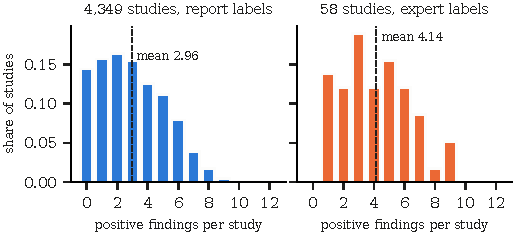
\includegraphics[width=\columnwidth]{figures/positives_per_study.pdf}
\caption{Number of positive findings per study: team-consensus labels (set~T, $\geq0.7$) of the 4,349 report-labelled studies
(left) and expert labels of the 58 reference studies (right). Dashed: mean.}
\label{fig:perstudy}
\end{figure}

\paragraph*{Report labellers versus expert labels} Fig.~\ref{fig:labellers} compares 12 public report-label tables with
the expert labels of \gold. Three further tables were flagged by the pipeline's heuristic (\gold{} macro AUC
$>0.995$, or ``gold'' in the source name; all three reached AUC 1.0). Perfect ranking does not prove that a table
contains the released reference labels, and we did not verify cell-by-cell equality; we treat them as potentially
reference-contaminated and conservatively excluded them. Macro AUCs of the remaining tables range from 0.81 to 0.91. Agreement is high for ACL, MCL,
medial meniscus and Baker's cyst (median 0.93--0.98) and lowest for synovitis (median 0.71), fracture (0.82), contusion
(0.83) and lateral OA (0.83), the findings for which reports are most often silent or hedged. The four tables averaged
into the reader's targets (Eq.~\ref{eq:v0}, marked $*$) span 0.82--0.89. With 58 studies, differences of a few hundredths
between tables are within sampling noise (Section~\ref{sec:res-yard}).

\begin{figure*}[!t]
\centering
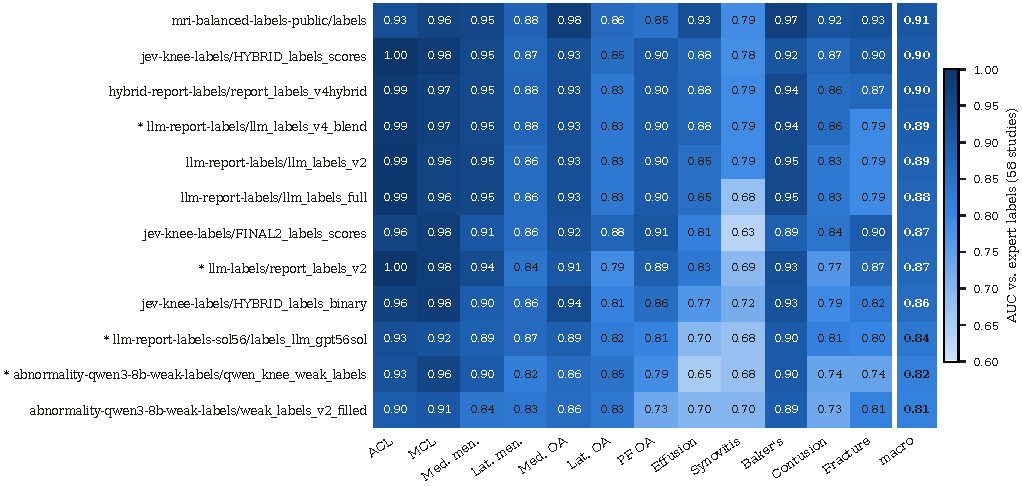
\includegraphics[width=0.92\textwidth]{figures/labeller_vs_expert.pdf}
\caption{Per-finding ROC AUC of public report-label tables against the expert labels of the 58 reference studies, sorted by
macro AUC (right column). $*$: the four tables averaged into the reader's targets v0. Three tables flagged as potentially
reference-contaminated are excluded; duplicate tables are shown once. Descriptive; $n=58$.}
\label{fig:labellers}
\end{figure*}

\subsection{Development and final-test partitions}
\label{sec:data-partitions}
Test labels are not released. A model is submitted as an offline inference program limited to 9~h on two NVIDIA T4 GPUs,
and the organisers' server computes the macro ROC AUC~\cite{hanley1982auc} (the mean over findings of the per-finding
AUC). Scores on a fixed 30\% partition (about 385 studies, displayed at three decimals) were visible during
development; we call this the \emph{development partition}. More than 60 configurations were scored on it, and its scores
informed which changes were kept, so it is not an independent test. Scores on the remaining 70\% (about 899 studies)
became visible only after all model and final-selection decisions had been made; we call this the \emph{final-test
partition}. It is a held-out evaluation not used for model development or final selection; we make no claim about
patient overlap with the training set or about the representativeness of the partition, which the organisers do not
report. Fig.~\ref{fig:dataflow} summarises how each part of the data was used.

\begin{figure*}[!t]
\centering
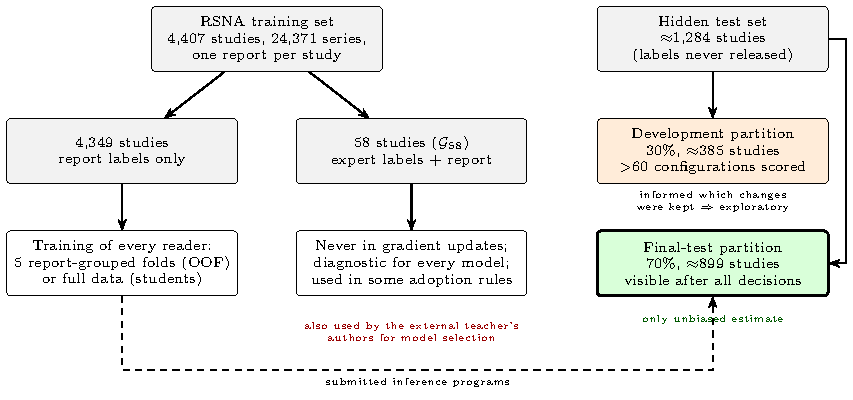
\includegraphics[width=0.82\textwidth]{figures/dataflow.pdf}
\caption{Use of the data. Left: the training set; every reader is trained on the 4,349 report-labelled studies, and the
58 expert-labelled studies serve as a development diagnostic. Right: the hidden test set; the development partition
informed model development, and the final-test partition was seen only after all decisions.}
\label{fig:dataflow}
\end{figure*} When two development scores display the same value, we used the
server's unrounded ordering of our own submissions; such orderings are ordinal and exploratory.

% =====================================================================================================
\section{Methods}
\label{sec:method}

Fig.~\ref{fig:overview} separates the reused components from those developed in this work. Let
$\mathcal{D}=\{(X_i,R_i)\}_{i=1}^{N}$ be the training studies with image series $X_i$ and report $R_i$, and
$\mathcal{C}$ the 12 findings. The goal is a scoring function $f:X\mapsto[0,1]^{12}$ whose per-finding rankings
maximise the macro AUC on unseen studies.



\subsection{Report-consensus targets}
\label{sec:method-labels}
We adopted the consensus construction of the public reader~\cite{goodpjw2026reader}, which averages four public LLM
label tables~\cite{labels2026public}: stevenleehans \texttt{llm\_labels\_v4\_blend}, pilkwang \texttt{report\_labels\_v2},
lixin73 \texttt{labels\_llm\_gpt56sol} and laymond \texttt{qwen\_knee\_weak\_labels}. We call the result \emph{v0}. With $y^{(s)}_{ic}\in[0,1]$ the label
of source $s$ for study $i$ and finding $c$, and $S_{ic}$ the sources that define it,
\begin{equation}
y^{\mathrm{rep}}_{ic}=\operatorname{clip}\!\Big(\tfrac{1}{|S_{ic}|}\textstyle\sum_{s\in S_{ic}} y^{(s)}_{ic},\;0.01,\;0.99\Big).
\label{eq:v0}
\end{equation}
We did not compare this consensus with each individual source under the same protocol, so we make no claim about its
benefit. Folds group studies with identical normalised report text (Algorithm~\ref{alg:labels}).

\begin{algorithm}[!t]
\caption{Report-consensus targets and report-grouped folds}
\label{alg:labels}
\begin{algorithmic}[1]
\Require studies $\mathcal{D}$, reports $R_i$; label tables $\{y^{(s)}\}_{s\in\mathcal{S}}$; reference set \gold; $K_f=5$
\Ensure targets $y^{\mathrm{rep}}\in[0.01,0.99]^{N\times12}$; fold index $\phi(i)\in\{-1,0,\dots,4\}$
\For{each study $i\notin$ \gold{} and finding $c$}
  \State $S_{ic}\gets\{s : y^{(s)}_{ic}\text{ defined}\}$;\; $y^{\mathrm{rep}}_{ic}\gets\operatorname{clip}\big(\operatorname{mean}_{s\in S_{ic}}y^{(s)}_{ic},0.01,0.99\big)$
\EndFor
\State $g_i\gets\textsc{Normalise}(R_i)$ \Comment{lower-case, strip non-alphanumerics}
\State $\phi\gets\textsc{GroupKFold}(K_f)$ on studies $\notin$ \gold{}, fixed permutation, groups $g_i$
\State $\phi(i)\gets-1$ for all $i\in$ \gold
\State \Return $y^{\mathrm{rep}},\phi$
\end{algorithmic}
\end{algorithm}

\subsection{Canonical preprocessing (reused)}
\label{sec:method-prep}
Each series is mapped to a canonical volume by one function shared by training and inference (Algorithm~\ref{alg:prep}).
Slices are ordered by position along the slice normal; each slice is transposed and flipped so that its rows and columns
follow the nearest canonical patient (LPS) axes. Oblique acquisitions are therefore re-oriented only to the nearest axis
and are not resampled into a common frame. Images are resampled to 0.4~mm pixels and centre-cropped to 153.6~mm
(384$\times$384 pixels). Intensities are windowed between the 1st and 99.5th percentiles, which are estimated on every
fourth pixel in each direction. Series are assigned to six slots by plane $\times$ fat suppression. Building the cache of
all training series produced no decoding errors; series with fewer than three slices are excluded.

\begin{algorithm}[!t]
\caption{Canonical volume for one DICOM series (reused)}
\label{alg:prep}
\begin{algorithmic}[1]
\Require slices $\{(I_j,\mathbf{o}_j,\mathbf{p}_j,\boldsymbol{\delta}_j)\}$ (pixels, orientation, position, spacing)
\Ensure uint8 volume $V\in\{0..255\}^{n\times384\times384}$, $n\le64$
\State invert MONOCHROME1; apply rescale slope and intercept
\State $\mathbf{n}\gets\mathbf{o}^{\mathrm{row}}\times\mathbf{o}^{\mathrm{col}}$;\; plane $\gets\arg\max_a|n_a|$
\State sort slices by $\sigma\,\langle\mathbf{p}_j,\mathbf{n}\rangle$ \Comment{$\sigma$: canonical direction}
\If{$n>64$} keep 64 uniformly spaced slices \EndIf
\For{each slice $j$}
  \State transpose/flip $I_j$ to the nearest canonical LPS axes
  \State crop the central $153.6\,\text{mm}$; resample to $0.4\,\text{mm}$; zero-pad to $384^2$
\EndFor
\State $(\ell,h)\gets$ percentiles $(1, 99.5)$ of $V[:,::4,::4]$
\State \Return $\operatorname{round}\big(255\cdot\operatorname{clip}((V-\ell)/(h-\ell),0,1)\big)$
\end{algorithmic}
\end{algorithm}

\subsection{2.5D multi-slot reader (reused)}
\label{sec:method-reader}
From each available slot $s$, $K$ window centres are spread over 4--96\% of the series (stratified-random in training,
uniform at evaluation); each centre $j$ gives a three-slice window $\mathbf{x}_{s,k}=[v_{j-1},v_j,v_{j+1}]$ encoded by an
ImageNet-pre-trained ConvNeXt-T or ConvNeXt-S~\cite{liu2022convnext,wightman2019timm}. Each feature is projected to
$d=384$ and tagged with a slot embedding and a position embedding:
$\mathbf{h}_{s,k}=\mathrm{LN}(W f(\mathbf{x}_{s,k}))+\mathbf{e}^{\mathrm{slot}}_{s}+g(p_{s,k})$. All $6K$ tokens pass
through a two-layer transformer encoder~\cite{vaswani2017attention}, and each finding has its own attention
pooling~\cite{ilse2018attention}:
\begin{align}
a_{c,n}&=\operatorname*{softmax}_n\big(\mathbf{u}_c^{\top}\tanh(V\mathbf{h}_n)\big),\\
z_c&=\mathbf{w}_c^{\top}\textstyle\sum_n a_{c,n}\mathbf{h}_n+b_c .
\end{align}
Fig.~\ref{fig:arch} shows the architecture and Algorithm~\ref{alg:reader} the forward pass.

\begin{figure*}[!t]
\centering
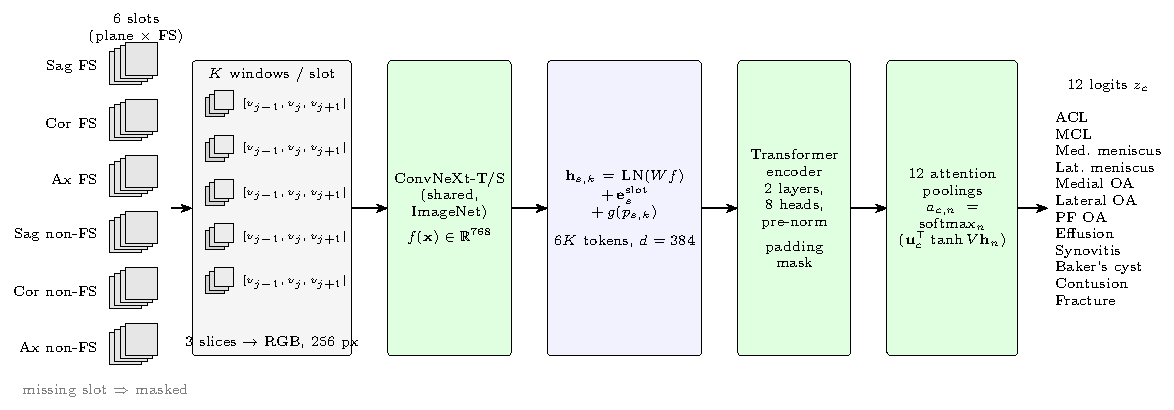
\includegraphics[width=\textwidth]{figures/architecture.pdf}
\caption{The reused 2.5D multi-slot reader~\cite{goodpjw2026reader}. Each available plane/fat-suppression slot contributes
$K$ three-slice windows; a shared ConvNeXt encodes each window, slot and slice-position embeddings are added, a two-layer
transformer mixes all tokens of the study, and one attention pooling per finding produces 12 logits. Missing slots are
masked.}
\label{fig:arch}
\end{figure*}

\begin{algorithm}[!t]
\caption{Forward pass of the 2.5D multi-slot reader (reused)}
\label{alg:reader}
\begin{algorithmic}[1]
\Require canonical volumes $\{V_s\}$ of one study; windows per slot $K$; training flag
\Ensure logits $\mathbf{z}\in\mathbb{R}^{12}$
\State $T\gets[\,]$
\For{each slot $s=1,\dots,6$ with a series}
  \State $\{j_k\}_{k=1}^{K}\gets$ \textsc{WindowCentres}$(|V_s|,K,\text{training})$
  \For{$k=1,\dots,K$}
    \State $\mathbf{x}\gets$ \textsc{View}$([V_s[j_k{-}1],V_s[j_k],V_s[j_k{+}1]])$ \Comment{crop, resize 256; jitter if training}
    \State append $\mathrm{LN}(Wf(\mathbf{x}))+\mathbf{e}^{\mathrm{slot}}_s+g(j_k/(|V_s|-1))$ to $T$
  \EndFor
\EndFor
\State $H\gets\textsc{Transformer}_{2}(T)$ \Comment{padding mask for missing slots}
\For{$c=1,\dots,12$}
  \State $\mathbf{a}_c\gets\operatorname{softmax}(\mathbf{u}_c^{\top}\tanh(VH^{\top}))$;\; $z_c\gets\mathbf{w}_c^{\top}(H^{\top}\mathbf{a}_c)+b_c$
\EndFor
\State \Return $\mathbf{z}$
\end{algorithmic}
\end{algorithm}

\subsection{Executed training configuration}
\label{sec:method-opt}
Every reader reported in Table~\ref{tab:distill} was trained by the released scripts listed in the Data and Code
Availability section with the configuration of Table~\ref{tab:hparams}. These scripts differ from the upstream reference
trainer in two respects: fp16 with loss scaling and gradient accumulation (the upstream trainer uses bf16 and direct
batches, which the T4 does not support efficiently). The kept checkpoint is the exponential moving average after the last
epoch, so no validation data select it. The EMA decay at update $t$ is $\min\big(0.998,(1+t)/(10+t)\big)$, a warm-up that
reaches 0.998 after about 4,000 updates. Augmentation is applied per series: rotation $\pm12^\circ$, scale $\pm12\%$,
translation $\pm6\%$, gamma and gain jitter.

\begin{table}[!t]
\centering
\caption{Executed training configuration of the 2.5D reader.}
\label{tab:hparams}
\setlength{\tabcolsep}{4pt}
\begin{tabular}{ll}
\toprule
Setting & Value\\
\midrule
Backbone & ConvNeXt-T / ConvNeXt-S, ImageNet\\
Parameters & 28M / 50M backbone + $\approx$3M head\\
Input & 6 slots $\times$ $K$ windows, 3 slices, 256 px\\
Windows $K$ & 8 (training), 12 (evaluation)\\
Head & $d=384$, 2 transformer layers, 8 heads\\
Optimiser & AdamW~\cite{loshchilov2019adamw}, weight decay 0.02\\
Learning rate & $10^{-4}$ backbone, $5\times10^{-4}$ head\\
Schedule & 1 warm-up epoch, cosine decay, 14 epochs\\
Batch & 8 studies = micro-batch 2 $\times$ 4 accumulation\\
Regularisation & drop-path 0.1, dropout 0.2, grad clip 3\\
Precision & fp16 with loss scaling\\
Weight averaging & EMA, decay $\min(0.998,\frac{1+t}{10+t})$\\
Hardware / time & 1 NVIDIA T4 per run, 5.6--7.9 h\\
\bottomrule
\end{tabular}
\end{table}

\subsection{Distillation targets and teacher provenance}
\label{sec:method-distill}
A student is trained on all 4,349 studies outside \gold{} with targets
\begin{equation}
\tilde{y}_{ic}=\operatorname{clip}\big((1-\tau)\,y^{\mathrm{rep}}_{ic}+\tau\,t_{ic},\;0.01,\;0.99\big),
\label{eq:mix}
\end{equation}
where $t_{ic}$ is a teacher probability and $\tau$ the teacher weight ($\tau=0$: report-only). A study the teacher did not
score keeps $y^{\mathrm{rep}}$. Table~\ref{tab:provenance} records what is known about each teacher. We call the external
teachers \emph{image-input} teachers: they read images, but most of their supervision is itself report-derived.

\begin{table*}[!t]
\centering
\caption{Teacher provenance. ``In-sample'': the teacher had been trained on the studies it labelled for the student.
Entries marked \emph{unverified} are as described by the component's authors and could not be checked against code or
data.}
\label{tab:provenance}
\footnotesize
\setlength{\tabcolsep}{3pt}
\begin{tabular}{p{2.3cm}p{3.0cm}p{3.6cm}p{2.5cm}p{2.6cm}p{2.4cm}}
\toprule
Teacher & Training images & Target labels & External data / pre-training & \gold{} use & Predictions used\\
\midrule
Self (arm B) & 4,349 RSNA studies, 5-fold CV & report consensus (Eq.~\ref{eq:v0}) & ImageNet only & diagnostic only; 3 of 5 fold models are public releases~\cite{goodpjw2026reader} & out-of-fold\\
Mirror (C, C2, C3, S75, T75s1) & 4,349 RSNA studies + 2,399 OAI knees~\cite{nartaa2026mirror} & RSNA: blend of report-derived label sets; OAI: expert MOAKS grades for PF OA, lateral OA, synovitis only (other cells masked) & OAI~\cite{peterfy2008oai}; ImageNet-pre-trained CoAtNet & excluded from training, used for selection; inference recipe tuned with development scores & in-sample\\
S1 component R6 (E75t, E75s) & RSNA training studies~\cite{heliosli2026blend} & \emph{unverified} & fastMRI auxiliary data~\cite{zbontar2018fastmri} (\emph{unverified}) & \emph{unverified} & reported as out-of-fold (\emph{unverified})\\
S1 component S6fall-B & all RSNA training studies~\cite{nartaa2026s6} & \emph{unverified} & SKM-TEA anatomy model~\cite{desai2021skmtea} & \emph{unverified} & in-sample (all-data model)\\
\bottomrule
\end{tabular}
\end{table*}

Because the external teachers were applied in-sample, their targets are not cross-fitted, and the student learns the
teacher's ranking of studies the teacher was fitted to. This does not leak hidden-test information, but it rules out
claims of fully cross-fitted supervision. Algorithm~\ref{alg:distill} gives the procedure.

\begin{algorithm}[!t]
\caption{Teacher--student distillation}
\label{alg:distill}
\begin{algorithmic}[1]
\Require targets $y^{\mathrm{rep}}$, folds $\phi$ (Alg.~\ref{alg:labels}); teacher type; weight $\tau$; seed
\Ensure student parameters $\theta_S$
\If{teacher is self}
  \For{$k=0,\dots,4$}
    \State train reader $\theta_k$ on $\{i: i\notin\text{\gold},\ \phi(i)\ne k\}$ with targets $y^{\mathrm{rep}}$
    \State $t_i\gets\sigma(f_{\theta_k}(X_i))$ for all $i$ with $\phi(i)=k$ \Comment{out-of-fold}
  \EndFor
\Else
  \State $t_i\gets$ \textsc{Teacher}$(X_i)$ for every $i\notin$ \gold \Comment{external model, in-sample}
\EndIf
\For{each $i\notin$ \gold}
  \State $\tilde{y}_i\gets\operatorname{clip}((1-\tau)y^{\mathrm{rep}}_i+\tau t_i,0.01,0.99)$ if $t_i$ defined, else $y^{\mathrm{rep}}_i$
\EndFor
\State initialise $\theta$ from ImageNet; $\bar\theta\gets\theta$; $t\gets0$
\For{epoch $=1,\dots,14$}
  \For{each batch $B\subset\{i\notin\text{\gold}\}$}
    \State $\mathcal{L}\gets\frac{1}{|B|}\sum_{i\in B}\mathrm{BCE}(f_\theta(X_i),\tilde{y}_i)$ \Comment{Alg.~\ref{alg:reader}}
    \State AdamW step on $\theta$; $t\gets t+1$; $d\gets\min(0.998,\frac{1+t}{10+t})$; $\bar\theta\gets d\,\bar\theta+(1-d)\,\theta$
  \EndFor
\EndFor
\State \Return $\theta_S\gets\bar\theta$
\end{algorithmic}
\end{algorithm}

\subsection{Rank-level fusion}
\label{sec:method-fusion}
Because the metric depends only on within-finding ranks, students are fused with an existing model or ensemble $P$ by
normalised ranks. With $r(\cdot)\in[0,1]$ the normalised rank over the test studies and $\bar{S}_{ic}$ the probability mean
of $M$ students,
\begin{equation}
F_{ic}=(1-w)\,r\big(P_{\cdot c}\big)_i+w\,r\big(\bar{S}_{\cdot c}\big)_i .
\label{eq:blend}
\end{equation}
$w=0.2$ was specified before the first fusion experiment, following a public notebook. Later, $w=0.3$ and $0.4$ were
evaluated on the development partition (four submissions on two parents); none ranked above the corresponding $w=0.2$
system, and $w=0.2$ was kept for every subsequent system. The inference safeguards (checkpoint hashes, time guard, fallback to the parent's
predictions, rank imputation for unscored studies) are given in Supplementary Algorithm~S1. Fused scores are ranks over a
cohort, not calibrated probabilities (Section~\ref{sec:discussion}).

% =====================================================================================================
\section{Experimental Setup}
\label{sec:setup}

\paragraph*{Implementation} PyTorch and timm~\cite{wightman2019timm}; training on single NVIDIA T4 GPUs (16~GB), two arms
in parallel on a two-GPU machine; a DICOM cache of all training series built in five CPU shards (53.6~GB).

\paragraph*{Protocol} Each experiment changed one variable relative to a parent with a known development score. Its
hypothesis and adoption rule were recorded in a version-controlled experiment log before the submission was scored
(for example, ``adopt if the stand-alone development AUC is at least the parent's $+0.003$ and \gold{} does not fall by
more than 0.01''). The log was not registered externally, so we describe it as prospectively logged rather than
pre-registered. It is released with the code~\cite{hack2publish2026repo}.

\paragraph*{Baselines} Eleven published methods for the same task whose inference code is public and whose development
score is displayed with the code~\cite{dread2026raptor,hengck2026mavit,mattiaangeli2026dino,jiweiliu2026fast,goodpjw2026stack,pjm2026d4,nartaa2026mirror,sujan2026apex,heliosli2026blend}.
We report their scores as published and did not re-train them.

\paragraph*{Statistics} \gold{} macro AUCs use 2,000 study-level bootstrap resamples~\cite{efron1993bootstrap}; a resample
in which a finding lacks positives or negatives contributes no AUC for that finding, and the macro AUC averages the
remaining findings. Patient identifiers are unavailable, so patient-level resampling was not possible. Paired differences
are computed on the same resamples. We do not interpret overlapping intervals or equal rounded scores as equivalence.

% =====================================================================================================
\section{Results}
\label{sec:results}

\subsection{Final-test partition}
\label{sec:res-final}
Table~\ref{tab:final} lists the comparisons that the final-test partition can answer. All model and selection decisions
were made before any final-test score was visible. The rows are grouped so that each comparison changes one thing:
stand-alone readers that differ only in the training target, and \emph{matched} ensemble pairs in which the same parent
was submitted with and without students. The two submitted final systems (the unchanged parent C2 and the fused system
H976, which adds students \emph{and} other switches) differ in several components, so their comparison is reported as a
system-level result and is not used as evidence for the students. H976 was the best of 23 configurations displayed at
0.958, so its development score is optimistically biased.

\begin{table}[!t]
\centering
\caption{Development (30\%) and final-test (70\%) macro AUC. The final-test partition was not used for development or
selection. ID: submission identifier.}
\label{tab:final}
\footnotesize
\setlength{\tabcolsep}{2.5pt}
\begin{tabular}{llcc}
\toprule
System & ID & Dev. & Final test\\
\midrule
\multicolumn{4}{l}{\emph{Stand-alone readers (target is the only change)}}\\
A: report targets & 57053758 & 0.933 & \TODO{}\\
B: self-distilled & 57053761 & 0.939 & \TODO{}\\
C: image-input teacher, $\tau=0.5$ & 57081442 & 0.948 & \TODO{}\\
C3: image-input teacher, $\tau=0.75$ & 57103459 & 0.949 & \TODO{}\\
Teacher alone~\cite{nartaa2026mirror} & -- & 0.949 & \TODO{}\\
\midrule
\multicolumn{4}{l}{\emph{Matched pairs (students are the only change)}}\\
P0: public CoAtNet + R6 blend & 57252502 & 0.958 & \TODO{}\\
\quad P0 + 5 Mirror students & 57281541 & 0.958 & \TODO{}\\
P1 = C2 (P0 + S6fall-B) & 57315983 & 0.958 & \TODO{}\\
\quad P1 + 5 Mirror students & 57369206 & 0.958 & \TODO{}\\
P1 + V2 weights & 57369271 & 0.958 & \TODO{}\\
\quad + 5 Mirror students & 57369477 & 0.958 & \TODO{}\\
P1 + V2 + BK + 5 students & 57447421 & 0.958 & \TODO{}\\
\quad + 2 S1 students & 57497105 & 0.958 & \TODO{}\\
\midrule
\multicolumn{4}{l}{\emph{Submitted final systems (several changes; system level only)}}\\
C2 (unchanged parent P1) & 57315983 & 0.958 & \TODO{}\\
H976 (P1 + V2 + BK + 7 students) & 57497105 & 0.958 & \TODO{}\\
\bottomrule
\end{tabular}
\end{table}

\TODO{Fill the final-test column from the Kaggle submission list (field privateScore) and describe the four matched pairs
and the A/B/C/C3 comparison here. If a row has no final-test score, say so; the corresponding development comparison then
remains exploratory. If a paired-difference figure is added, plot final-test minus development differences per pair.}

\subsection{Training targets (development partition)}
\label{sec:res-distill}
Table~\ref{tab:distill} and Fig.~\ref{fig:leg} list every full-data reader; each differs from its parent in one variable.

\begin{table}[!t]
\centering
\caption{Full-data 2.5D readers. $\tau$: teacher weight in (\ref{eq:mix}). \gold: descriptive (Section~\ref{sec:data-gold}).
Dev.: stand-alone development-partition AUC; ``--'' not evaluated alone.}
\label{tab:distill}
\footnotesize
\setlength{\tabcolsep}{2pt}
\begin{tabular}{lllccc}
\toprule
Arm & Backbone & Target & $\tau$ & \gold & Dev.\\
\midrule
A & ConvNeXt-T & reports & 0 & 0.907 & 0.933\\
B & ConvNeXt-T & + self OOF & 0.5 & 0.904 & 0.939\\
B2 & ConvNeXt-T in22k & + self OOF & 0.5 & 0.907 & 0.938\\
\midrule
C & ConvNeXt-T & + Mirror & 0.5 & 0.923 & 0.948\\
C2 & ConvNeXt-T (seed 1) & + Mirror & 0.5 & 0.919 & 0.948\\
C3 & ConvNeXt-T & + Mirror & 0.75 & 0.927 & 0.949\\
S75 & ConvNeXt-S & + Mirror & 0.75 & 0.921 & --\\
T75s1 & ConvNeXt-T (seed 1) & + Mirror & 0.75 & 0.931 & --\\
\midrule
E75t & ConvNeXt-T & + S1 ens. & 0.75 & 0.926 & --\\
E75s & ConvNeXt-S & + S1 ens. & 0.75 & 0.924 & --\\
\midrule
\multicolumn{4}{l}{Mean of 5 Mirror students} & 0.926 & --\\
\multicolumn{4}{l}{Mean of 5 Mirror + 2 S1 students} & 0.928 & --\\
\bottomrule
\end{tabular}
\end{table}

\begin{figure}[!t]
\centering
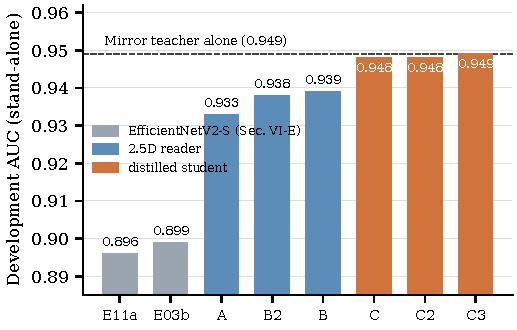
\includegraphics[width=\columnwidth]{figures/leg_alone.pdf}
\caption{Stand-alone development-partition AUC of each model. E11a and E03b are the EfficientNetV2-S models of
Section~\ref{sec:res-own}. The dashed line is the image-input teacher's displayed score.}
\label{fig:leg}
\end{figure}

\paragraph*{Observed} Self-distillation (B vs A) raised the development AUC from 0.933 to 0.939; replacing the
self-teacher by the image-input teacher (C vs B) raised it to 0.948, and $\tau=0.75$ (C3) displayed 0.949, the same value
as the teacher at three-decimal precision. On \gold, B differed from A by $-0.003$, and C from B by $+0.019$, with the largest
per-finding changes on synovitis (0.717$\to$0.791) and fracture (0.844$\to$0.933). No clear benefit was observed from
ImageNet-22k pre-training (B2 vs B, $-0.001$), from ConvNeXt-S (S75 vs C3 on \gold; also $-0.003$ and $-0.004$ OOF in an
earlier cross-validated comparison with report targets), or from a second seed (C2 vs C, equal at three decimals). Only
two seeds were run, so seed variability is not characterised.

\paragraph*{Caveats} These are development-partition comparisons and, until confirmed on the final-test partition, are
exploratory. The \gold{} changes of the Mirror students are not independent, because the teacher's authors selected it on
\gold. Three explanations for the C-vs-B gain are confounded and are not separated by our experiments: image evidence
learned by the teacher, external data (OAI with expert grades for three findings), and complementary errors between
teacher and reader. A teacher-only target ($\tau=1$) and a teacher matched in architecture but without external data were
not run.

\paragraph*{Cost} We make no claim about inference cost: measured runtimes are not available for either the teacher or
the students. (The teacher's authors report submit-to-score turnaround, which includes queueing and is explicitly not
an inference runtime~\cite{nartaa2026mirror}.) \TODO{Add measured per-study decode time, model time, peak memory and
fallback counts for a single student and for the seven-student stage, from the inference logs.}

\subsection{Comparison with published methods (development partition)}
\label{sec:res-compare}
Table~\ref{tab:compare} places the readers among published methods evaluated on the same development partition. A single
distilled reader displayed the same AUC as the best published single model, the teacher it was distilled from. Because
published scores were also obtained with development feedback, the table is descriptive.

\begin{table}[!t]
\centering
\caption{Development-partition macro AUC of published methods (as displayed with their code) and of this work.
$\dagger$: uses weights trained with external data (OAI, fastMRI or SKM-TEA). Descriptive only.}
\label{tab:compare}
\footnotesize
\setlength{\tabcolsep}{2.5pt}
\begin{tabular}{p{5.2cm}c}
\toprule
Method & Dev. AUC\\
\midrule
\multicolumn{2}{l}{\emph{Published single models}}\\
CoAtNet MIL, report labels~\cite{dread2026raptor} & 0.924--0.932\\
MaViT~\cite{hengck2026mavit} & 0.935\\
Anatomical-mirror CoAtNet MIL$^\dagger$~\cite{nartaa2026mirror} & 0.949\\
\midrule
\multicolumn{2}{l}{\emph{Published ensembles}}\\
DINOv2/DINOv3/RadImageNet/CoAtNet blend~\cite{mattiaangeli2026dino} & 0.941\\
Re-weighted blend + extra readers~\cite{jiweiliu2026fast} & 0.943\\
Stack + 2.5D ConvNeXt MIL~\cite{goodpjw2026stack} & 0.944\\
+ private EffNetV2-S/CoAtNet/ConvNeXt-L leg~\cite{pjm2026d4} & 0.946\\
Mirror + 2.5D reader stack$^\dagger$~\cite{sujan2026apex} & 0.950\\
Mirror + compact ConvNeXt (S6)$^\dagger$~\cite{heliosli2026blend} & 0.954\\
Mirror + compact ConvNeXt (R7)$^\dagger$~\cite{heliosli2026blend} & 0.956\\
CoAtNet 384/224 + R6 blend$^\dagger$~\cite{heliosli2026blend,goodpjw2026stack} & 0.958\\
\midrule
\multicolumn{2}{l}{\emph{This work}}\\
Reader, report targets (A) & 0.933\\
Reader, self-distilled (B) & 0.939\\
Reader, image-input teacher (C3)$^\dagger$ & 0.949\\
Final fused system$^\dagger$ & 0.958\\
\bottomrule
\end{tabular}
\end{table}

\subsection{Fusion with existing ensembles (development partition)}
\label{sec:res-ens}
Table~\ref{tab:ens} lists every comparison in which the students were the only change to an existing ensemble. Three
comparisons changed the displayed score (0.954$\to$0.955 once, 0.956$\to$0.957 twice, with three and with five students on
the same parent); in the remaining five the displayed score was unchanged and the unrounded ordering placed the fused variant above its parent. These are eight ordinal, non-independent
comparisons on the same partition---they share parents and students---so we report them as consistent with a small benefit
that requires final-test confirmation, not as an established improvement. Further single-change switches inside the
ensembles are reported in Supplementary Table~S1.

\begin{table}[!t]
\centering
\caption{Students as the single change to an existing ensemble (Eq.~(\ref{eq:blend}), $w=0.2$), development partition.
``$>$'': ranked above the parent in the unrounded ordering (ordinal, exploratory).}
\label{tab:ens}
\footnotesize
\setlength{\tabcolsep}{2.5pt}
\begin{tabular}{llcc}
\toprule
Parent ensemble & Added & Parent & Fused\\
\midrule
Mirror + S6 compact & C & 0.954 & 0.955\\
Mirror + R7 compact & C, C2, C3 & 0.956 & 0.957\\
Mirror + R7 compact & 5 Mirror st. & 0.956 & 0.957\\
CoAtNet + R6 blend & 5 Mirror st. & 0.958 & 0.958 ($>$)\\
+ S6fall-B (P1) & 5 Mirror st. & 0.958 & 0.958 ($>$)\\
P1 + V2 weights & 5 Mirror st. & 0.958 & 0.958 ($>$)\\
P1+V2+BK + 5 st. & 2 S1 st. & 0.958 & 0.958 ($>$)\\
P1+BK+FK + 5 st. & 2 S1 st. & 0.958 & 0.958 ($>$)\\
\bottomrule
\end{tabular}
\end{table}

\subsection{Negative results: EfficientNetV2-S on a published corpus}
\label{sec:res-own}
Before the reader, we trained EfficientNetV2-S~\cite{tan2021efficientnetv2} at 384~px with stochastic weight
averaging~\cite{izmailov2018swa} on a published 44-slice corpus and its labels~\cite{dread2026raptor} (E11). Two folds
reached an OOF AUC of 0.872 (soft-label estimand, Table~\ref{tab:own}) and \gold{} 0.900, but the model alone displayed
0.896, and adding it at a prospectively logged weight of 0.30 lowered a 0.943 ensemble to 0.935. A test-time preprocessing
mismatch was excluded by rebuilding 218 training studies from DICOM: pixels matched, prediction ranks agreed on all 12
findings, and \gold{} AUC was identical. A four-source consensus target (E03b) displayed 0.899, and a ResNet-34 multi-view
model on our own cache (E13) had a lower OOF AUC (0.843). Better OOF did not imply a useful ensemble member: the model shared
data, labels and head design with the ensemble's dominant component.

\begin{table}[!t]
\centering
\caption{EfficientNetV2-S@384 models (two folds). OOF: pooled over 1,740 studies against the soft training labels, with
labels in the uncertain band 0.25--0.7 excluded ($^{\dagger}$consensus labels; 0.873 against the labels of E11).}
\label{tab:own}
\footnotesize
\setlength{\tabcolsep}{3.5pt}
\begin{tabular}{llccc}
\toprule
ID & Change & OOF & \gold & Dev.\\
\midrule
-- & published ensemble (parent) & -- & -- & 0.943\\
E11 & parent + model, $w=0.30$ & 0.872 & 0.900 & 0.935\\
E11a & model alone & 0.872 & 0.900 & 0.896\\
E03b & alone, consensus labels & 0.911$^{\dagger}$ & 0.883 & 0.899\\
E13 & ResNet-34, own cache & 0.843 & 0.865 & --\\
\bottomrule
\end{tabular}
\end{table}

Table~\ref{tab:perfind} gives E11's per-finding OOF AUC under a different estimand (labels binarised at 0.5, no band
excluded; macro 0.870). Lateral meniscus, contusion, lateral OA and PF OA had the lowest agreement with report labels.

\begin{table}[!t]
\centering
\caption{Per-finding OOF AUC of E11 against report labels binarised at 0.5 (folds 0+1, $n=1{,}740$, no band excluded;
macro 0.870) and positives in \gold.}
\label{tab:perfind}
\footnotesize
\setlength{\tabcolsep}{3pt}
\begin{tabular}{lcc@{\hskip 8pt}lcc}
\toprule
Finding & OOF & $n_+$ & Finding & OOF & $n_+$\\
\midrule
ACL & 0.890 & 24 & PF OA & 0.845 & 21\\
MCL & 0.846 & 9 & Effusion & 0.908 & 35\\
Med. meniscus & 0.894 & 26 & Synovitis & 0.891 & 27\\
Lat. meniscus & 0.816 & 23 & Baker's cyst & 0.926 & 12\\
Medial OA & 0.885 & 15 & Contusion & 0.813 & 19\\
Lateral OA & 0.832 & 11 & Fracture & 0.896 & 18\\
\bottomrule
\end{tabular}
\end{table}

\subsection{Resolution of the development yardsticks}
\label{sec:res-yard}
\paragraph*{\gold} For E11, the \gold{} macro AUC of 0.900 has a 95\% bootstrap interval of [0.872, 0.924]; for E03b,
0.883 has [0.846, 0.915]; their paired difference of $-0.017$ has [$-0.042$, $+0.003$]. These intervals describe E11 and
E03b, whose \gold{} predictions are stored; the predictions of A, B and C3 on \gold{} were not retained locally, so paired
intervals for the principal comparisons are not reported. \TODO{Required before submission: download
\texttt{gold\_arm\{A,B,C,C3\}.csv} from the training-kernel outputs and report the paired intervals for B$-$A, C$-$B and
C3$-$A computed by the released script; they remain descriptive because \gold{} was used in development.}

\paragraph*{Development partition (illustration)} To illustrate how much a 385-study partition can resolve, we used
E11's OOF predictions (1,740 studies, report labels binarised at 0.5) as a stand-in population. Under these assumptions,
the macro AUC of a fixed model has a standard deviation of 0.0085 across random 385-study subsets (Fig.~\ref{fig:noise}).
We then created a second model by adding Gaussian noise to E11's predictions, so that its full-sample AUC was lower by a
known gap, and counted how often a subset ordered the two wrongly: gaps of 0.0003, 0.0012 and 0.0037 were mis-ordered 25\%,
10\% and 2\% of the time. These rates depend on the chosen model, perturbation, prevalence, correlation between models and
label noise; they illustrate, rather than estimate, the resolution of the hidden partition. Repeated comparisons on the
same partition are not independent replications.

\begin{figure}[!t]
\centering
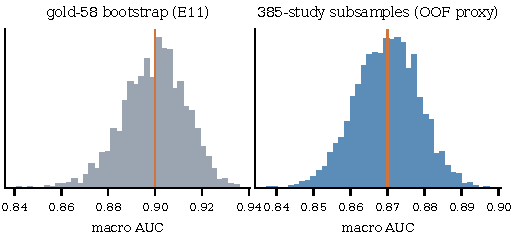
\includegraphics[width=\columnwidth]{figures/yardstick_noise.pdf}
\caption{Illustration of yardstick resolution. Left: bootstrap distribution of E11's \gold{} macro AUC. Right: macro AUC of
the same model on random 385-study subsets of its OOF predictions (report labels). Vertical lines: full-sample values.}
\label{fig:noise}
\end{figure}

% =====================================================================================================
\section{Discussion}
\label{sec:discussion}

\paragraph*{Findings} On the development partition, the training target was associated with larger differences than the
backbone, pre-training or seed in the configurations we evaluated; distillation from an image-input teacher gave the largest
change, and fused students ranked above their parent ensembles in every development comparison. Whether these differences
hold on the final-test partition is reported in Section~\ref{sec:res-final}.

\paragraph*{Possible explanations (not tested)} The teacher may encode image evidence that reports omit; it was also
trained with external data that include expert grades for three findings, and teacher and reader may make complementary
errors. Our experiments do not separate these mechanisms (Section~\ref{sec:res-distill}). The development gain of fused
students may reflect the different representation of the reader or the report term in (\ref{eq:mix}), which keeps the
student partly anchored to reports.

\paragraph*{Relation to prior work} Kooklan~\cite{kooklan2026gap} found that a report--image mixture agreed better with the
expert labels than either source, but did not improve a 2.5D ResNet-50 on the final-test partition. Our development gains
point the other way; the final-test scores of our readers are needed before concluding that the difference reflects the
reader, the teacher, or development-partition over-fitting.

\paragraph*{Clinical considerations} A macro AUC around 0.95 on the development partition does not establish clinical
usefulness. Clinical prioritisation is a potential application that would require per-finding sensitivity and specificity
at thresholds fixed on development data, precision--recall analysis for uncommon findings, calibration, review of false
positives and negatives by a qualified reader, and subgroup and scanner analyses on an independent cohort with compatible
label definitions. Rank-fused scores are not probabilities, and their values depend on the cohort being ranked; a single
newly arriving examination would require either a reference cohort against which to rank it or the students' own
(uncalibrated) probabilities.

\paragraph*{Ethical and data considerations}
\label{sec:ethics}
The dataset is de-identified and was used under its terms of use. \TODO{State whether your institution required ethics
review or granted an exemption.} Components marked $\dagger$ were trained by their authors with external research data
(OAI, fastMRI or SKM-TEA; Table~\ref{tab:provenance}); the dataset's rules allowed external data only under conditions that
each participant had to verify. Our results without such weights are the report-target reader A (0.933) and the
self-distilled reader B (0.939).

% =====================================================================================================
\section{Limitations}
\label{sec:limitations}
(i) Except Table~\ref{tab:final}, all scores come from a 385-study development partition that informed development; they
are exploratory. (ii) \gold{} is small and enriched, was used in adoption rules, and was used by the teacher's authors for
selection. (iii) External teachers were applied in-sample, and their provenance is partly unverified
(Table~\ref{tab:provenance}). (iv) Ablations needed to explain the main gain were not run: teacher-only targets ($\tau=1$), a
teacher without external data, at least three seeds of A, B and C3, and individual label sources versus their consensus.
(v) Institutions, acquisition period, demographics, scanners, inclusion criteria, patient identifiers and the
selection of \gold{} were not reported by the organisers (label definitions and the reading procedure were;
Table~\ref{tab:defs}). (vi) No external testing,
calibration or reader study was performed. (vii) The fused system depends on published models whose training we could
only partly audit.

% =====================================================================================================
\section{Conclusion}
\label{sec:conclusion}
For a report-supervised 2.5D knee MRI reader with 58 expert-labelled studies, changing the training target from report
consensus to a mixture with an image-input teacher was associated with a development-partition AUC increase from 0.933 to
0.949, while the backbone, pre-training and seed changes we evaluated showed no clear benefit; students fused with
existing ensembles ranked above their parents in all development comparisons. These findings are exploratory until
confirmed on the final-test partition (Section~\ref{sec:res-final}) and on external data, and the mechanism of the gain
remains to be isolated with teacher-only and external-data-matched controls.

% =====================================================================================================
\section*{Data and Code Availability}
The dataset is available from the RSNA under its terms of use~\cite{rsna2026knee}. Code, the executed training scripts of all
readers except the two S1 students (\TODO{add the script of Kaggle kernel \texttt{hosen42/rsna-knee-gpjw-student5}}),
inference scripts, fold assignments, the experiment log and the scripts that regenerate all figures are at
\url{https://github.com/hamidhosen42/RSNA-Knee-Abnormality-Detection} (folder \texttt{ieee\_access\_paper},
\TODO{tag a release and cite its version/DOI}). \TODO{State where trained checkpoints (with SHA-256) can be obtained.}
Published components remain under their authors' licences.

\section*{Use of AI Tools}
\TODO{Confirm and adapt:} Portions of the manuscript text, figures and analysis code were drafted with the assistance of
an AI system (Claude, Anthropic). The authors reviewed and edited all content and take full responsibility for it.

\section*{Acknowledgment}
The authors thank the RSNA for releasing the dataset and the authors of the published models, labels and code used in this
study: goodpjw2008 (2.5D reader), dreaddevelopment (CoAtNet MIL models and corpus), nartaa (Mirror and S6fall-B models),
heliosli (compact ConvNeXt bundles and ensembles), hengck23 (MaViT), and stevenleehans, pilkwang, lixin73 and laymond
(report label tables). \TODO{Add institutional acknowledgments.}

\bibliographystyle{IEEEtran}
\bibliography{references}

% ----- IEEE Access requires a biography and a photo for every author; replace with
% \begin{IEEEbiography}[{\includegraphics[width=1in,height=1.25in,clip,keepaspectratio]{photo.png}}]{Name} -----
\begin{IEEEbiographynophoto}{Md. Hamid Hosen}
\TODO{Biography (about 100 words) and photo.}
\end{IEEEbiographynophoto}

\begin{IEEEbiographynophoto}{Md. Foysal Emon Shanto}
\TODO{Biography and photo.}
\end{IEEEbiographynophoto}

\begin{IEEEbiographynophoto}{Md Esfer Abdus Sami}
\TODO{Biography and photo.}
\end{IEEEbiographynophoto}

\begin{IEEEbiographynophoto}{\TODO{Author 4 (kishormorol)}}
\TODO{Biography and photo.}
\end{IEEEbiographynophoto}

\EOD

\end{document}
